\documentclass[10pt,a4paper]{article}
\usepackage[margin=2.1cm]{geometry}
\usepackage{amsmath,amssymb,booktabs,graphicx,xcolor,microtype}
\usepackage[hidelinks]{hyperref}
\usepackage{caption}
\captionsetup{font=small,labelfont=bf}
\setlength{\parskip}{3pt}
\newcommand{\code}[1]{\texttt{#1}}

\title{\vspace{-1.2cm}\textbf{Language-Conditioned Pick-and-Place in Simulation:\\
a Clearance-Aware Grasp Pipeline and a Study of Cross-Attention Pooling}}
\author{Sattwik Singh\\ \small Department of Electrical Engineering, IIT Delhi\\
\small Code: \url{https://github.com/Sattwik-Singh/grasp-vla}}
\date{\small November 2026}

\begin{document}
\maketitle
\vspace{-0.6cm}

\begin{abstract}
\noindent I build and evaluate, in an open simulation, a
language-conditioned pick-and-place system. A Franka Panda in PyBullet
parses an instruction, detects objects in an overhead RGB-D image, decides which
one is meant, and grasps it with a clearance-aware planner. On 200 unseen scenes
per condition, the pipeline succeeds in 99--100\% of episodes across clean,
cluttered, noisy-sensor, low-friction and combined conditions. Ablations show
that splitting touching objects by colour removes almost all wrong-object
errors (success 90.5\%$\rightarrow$99.0\% in the hardest condition).
A stress sweep shows the real weak point is camera calibration: success falls
to 71\% at 15\,mm of error. Object spacing, even down to 1\,mm, barely matters.
In a controlled comparison of four ways to pool object tokens in a learned
grounding policy, cross-attention pooling with an instruction-derived query
cuts the correlation between representations of different instructions by 63\%
(0.951$\rightarrow$0.348) and is the only variant that learns the task within the same 12-epoch budget
(98.7\% grounding accuracy against a 16.8\% chance level; an instruction-modulated
mean pool reaches 61\% after 40 epochs). Inside the robot loop it
completes 94\% of cluttered episodes. I also report where the system fails
and what this setup cannot show.
\end{abstract}

\section{Introduction}
Robots that follow natural-language instructions usually chain several parts:
a detector that finds objects, often open-vocabulary~\cite{owlvit,clip}; a
planner that turns the instruction into steps, sometimes an LLM~\cite{saycan};
a grounding step that decides which object is meant; and a grasp planner.
End-to-end vision-language-action (VLA) policies~\cite{cliport,rt2} fold
grounding into a learned model, where a key design choice is how the image
features are pooled together with the instruction. This independent study builds such a
system in an open, fully reproducible simulation and measures it under
controlled conditions. Two questions guide the work:
\begin{enumerate}\itemsep0pt
\item[\textbf{Q1}] How reliable is a modular \emph{instruction $\rightarrow$
detect $\rightarrow$ ground $\rightarrow$ grasp} pipeline, and where does it fail?
\item[\textbf{Q2}] Does cross-attention pooling make a policy's internal
representation instruction-specific, and does that translate into choosing
the right object?
\end{enumerate}
All numbers below come from scripts in the repository, run on fresh random
scenes whose seeds were never used during development.


\section{Simulation setup}
\textbf{Scene.} A Franka Panda arm in PyBullet~\cite{pybullet} stands at the edge
of a table with a tray. Each scene places 5 or 8 objects at random positions and
orientations. Each object is a cube, an upright cylinder or a ball (radius or
half-size 2.0--2.8\,cm, mass 50--200\,g) in one of six colours, and no
colour--shape pair appears twice in a scene. A fixed overhead camera gives a
$320{\times}320$ RGB-D image. The simulator's segmentation masks and true
poses are used only to \emph{score} episodes; the robot never sees them.

\textbf{Instructions.} Instructions are drawn from templates with synonyms
(``block'', ``can'', ``marble'', \ldots), e.g.\ \emph{``grab the blue tube and
drop it in the basket''}. A quarter name two objects (\emph{``move the green
marble to the bin, then the red cylinder''}).

\textbf{Conditions.} Five conditions test different failure sources:
\emph{clean} (5 objects, at least 3\,cm apart); \emph{clutter} (8 objects,
gaps down to 8\,mm); \emph{sensor noise} (2\,mm depth noise plus an unknown
camera offset with 6\,mm standard deviation, so the perception code works with
a miscalibrated camera); \emph{low friction} ($\mu\in[0.3,0.6]$); and
\emph{combined} (all of the above, $\mu\in[0.4,1.0]$).

\textbf{Success.} A step succeeds if the named object is lifted at least 10\,cm,
held for one simulated second, and ends up inside the tray. An episode succeeds
only if every step succeeds. Failed steps are labelled \emph{parse failure},
\emph{no detection}, \emph{wrong object}, \emph{grasp miss}, \emph{drop} or
\emph{place miss}.

\textbf{Seeds.} Development used scene seeds 0--39, a pilot on 1000--1029
(which exposed merged detections), and a first full run on 2000--2199 (whose
grasp failures motivated the clearance-aware planner). All reported pick-and-place results use seeds 3000--3199, the stress
sweep 5000--5099 and the learned-policy loop 4000--4099.

\section{The modular pipeline}
\textbf{Planner.} A rule-based parser turns the instruction into a list of
\emph{(colour, shape)} targets and decides whether to place them in the tray.
The repository also contains a drop-in LLM planner that returns the same JSON
plan, but it is not used in any reported result, so every number is
reproducible offline.

\textbf{Detection.} The depth image is back-projected to world points. Points
more than 6\,mm above the table, outside the tray, are grouped into connected
components. Touching objects merge into one component, so each component is
split by 2-means clustering on pixel chromaticity when the two cluster centres
are clearly apart (\emph{colour splitting}, applied recursively). This step
uses no colour names. Each detection yields a grasp point, the angle of its
smallest enclosing rectangle and an RGB crop.

\textbf{Grounding.} The default grounder labels each detection's colour by
nearest chromaticity and its shape from two geometric cues: how much of its
bounding rectangle the footprint fills (squares $\approx$0.90, discs
$\approx$0.79) and how domed its top is. The thresholds were tuned on the
development scenes. An open-vocabulary CLIP~\cite{clip} grounder that scores
image crops against the phrase is implemented, but its weights could not be
downloaded in the compute environment I used, so it is not evaluated here.

\textbf{Grasp planning.} The \emph{simple} planner aligns the gripper with the
object's rectangle and opens the fingers fully (4\,cm each side). The
\emph{clearance-aware} planner opens the fingers only to the object's width
plus 1.2\,cm. It then tries candidate wrist angles (the two face-aligned angles
for boxes, 15$^\circ$ steps for round objects) and keeps the angle whose finger
footprints overlap the fewest points from neighbouring objects in the height
map. The arm then moves in Cartesian straight lines using inverse kinematics.

\section{Learned grounding and cross-attention pooling}
To study the pooling question in isolation, I trained a small language-conditioned
grounding policy. It sees one token per detected object (a CNN on the object's
$24{\times}24$ RGB-D crop plus an MLP on its position, followed by
LayerNorm). It encodes the instruction with a bidirectional GRU, and predicts
the table position of the object to pick. The object tokens are pooled into one
vector $v$, the fused representation is $h=\mathrm{MLP}([v;\ell])$, where
$\ell$ is the language vector, and a linear head maps $h$ to $(x,y)$. Only the
pooling step differs between the four variants:
\begin{itemize}\itemsep0pt
\item \textbf{Mean}: $v$ is the average token, so it is the same for every instruction.
\item \textbf{Attention (learned query)}~\cite{settransformer}: attention with a
fixed learned query. It has the same capacity as cross-attention, but its
pooling still ignores the instruction.
\item \textbf{FiLM + mean}~\cite{film}: every token is scaled and shifted by
the instruction before mean pooling. This is a stronger instruction-aware
baseline.
\item \textbf{Cross-attention}~\cite{attention}: the attention query is a
projection of $\ell$, so the instruction decides how much each object
contributes.
\end{itemize}

\textbf{Cross-instruction correlation.} For a test scene with $K$ objects, I
encode the same scene under the $K$ instructions that name each object, and
average the pairwise Pearson correlations between the resulting fused
vectors $h_1,\dots,h_K$:
\[
\rho=\frac{1}{K(K-1)}\sum_{i\neq j}\operatorname{corr}(h_i,h_j).
\]
A value near 1 means the representation barely changes with the instruction,
which suggests the policy is not really listening. Since a low
correlation is only useful if the policy picks the right object, I also report
\emph{grounding accuracy}, the fraction of test instructions for which the
object nearest the predicted point is the named one.

\textbf{Data and training.} 2000 training scenes (12\,070 instructions) and
300 test scenes (1\,785 instructions), each with 4--8 objects and gaps of
8--30\,mm. Each variant is trained for 12 epochs (AdamW, one-cycle learning
rate peaking at $10^{-3}$, MSE loss) with three seeds, on a 2-core CPU.


\section{Results}
\subsection{Pick-and-place (Q1)}
\begin{figure}[t]
\centering
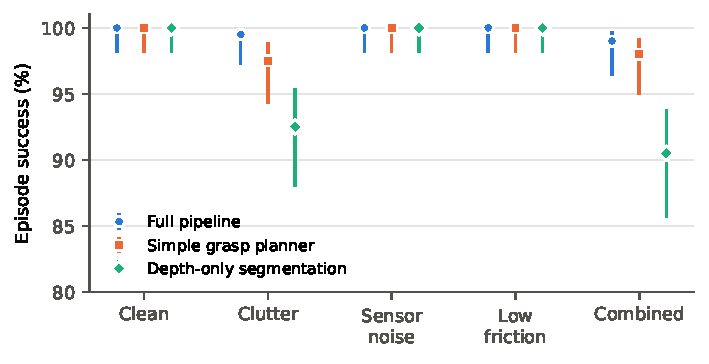
\includegraphics[width=0.78\linewidth]{figures/grasp_success.pdf}
\caption{Episode success on 200 unseen scenes per condition (seeds 3000--3199),
with 95\% Wilson intervals. Blue: full pipeline. Orange: simple grasp planner.
Green: depth-only segmentation (no colour splitting).}
\label{fig:grasp}
\end{figure}

\begin{table}[t]
\centering\small
\begin{tabular}{lccc}
\toprule
Condition & Full pipeline & Simple grasp planner & Depth-only segmentation\\
\midrule
Clean & 100\% & 100\% & 100\%\\
Clutter & \textbf{99.5\%} [97.2, 99.9] & 97.5\% [94.3, 98.9] & 92.5\% [88.0, 95.4]\\
Sensor noise & 100\% & 100\% & 100\%\\
Low friction & 100\% & 100\% & 100\%\\
Combined & \textbf{99.0\%} [96.4, 99.7] & 98.0\% [95.0, 99.2] & 90.5\% [85.6, 93.8]\\
\midrule
\multicolumn{4}{l}{\emph{Failed steps in clutter (254 steps):}}\\
\quad wrong object / grasp miss & 1 / 0 & 1 / 4 & 14 / 1\\
\bottomrule
\end{tabular}
\caption{Pick-and-place success (200 episodes per cell, 54 of them with two
targets; 95\% intervals in brackets). No episode failed through parsing, a
missed detection, a drop or a missed placement.}
\label{tab:grasp}
\end{table}

Figure~\ref{fig:grasp} and Table~\ref{tab:grasp} show that the full pipeline
succeeds in 99--100\% of episodes in every condition. Three findings stand out.
(i) \textbf{Clutter is the only condition that causes failures}; sensor noise,
camera miscalibration of a few millimetres and low friction cause none.
(ii) \textbf{Colour splitting matters most.} Without it, touching objects merge
into one detection and the robot picks the wrong one: wrong-object steps rise
from 1 to 14 in clutter and from 1 to 18 in the combined condition, and success
drops by 7--8.5 points. (iii) \textbf{The clearance-aware planner} reduces
grasp misses in clutter (4 to 0) and in the combined condition (3 to 1), but the
difference is inside the confidence intervals. Section~\ref{sec:stress} pushes
spacing and calibration further to show where each version breaks.

\subsection{Where does it break?}\label{sec:stress}
\begin{figure}[t]
\centering
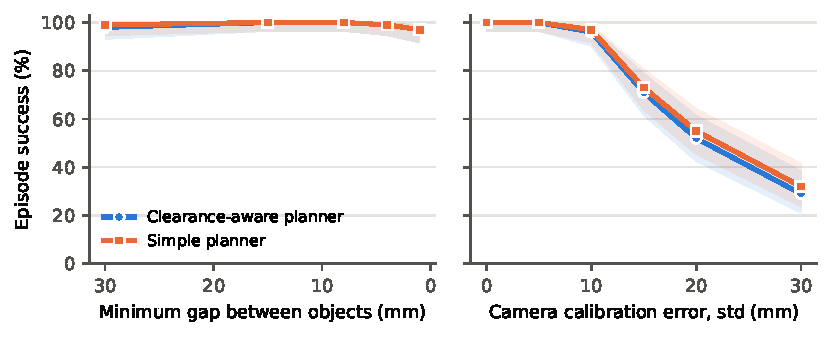
\includegraphics[width=0.82\linewidth]{figures/stress.pdf}
\caption{Stress sweep, 100 unseen scenes per point (seeds 5000--5099), with 95\%
intervals. Left: 8 objects packed ever more tightly. Right: 5 objects with an
increasing unknown camera offset.}
\label{fig:stress}
\end{figure}
Figure~\ref{fig:stress} varies one difficulty knob at a time. \textbf{Spacing
barely matters}: even with gaps of 1\,mm between eight objects, success stays at
97\%, and the few failures are wrong-object choices between touching objects of
similar colour. \textbf{Camera calibration is the real weak point.} Success is
100\% up to 5\,mm of error, 96\% at 10\,mm, 71\% at 15\,mm and 29\% at 30\,mm,
and almost every failure is a grasp miss. The system trusts the camera's
geometry completely and has no feedback (such as a wrist camera or a re-grasp)
to correct a misplaced gripper.

The two grasp planners behave almost identically in both sweeps. Pooling the
two hardest conditions of Table~\ref{tab:grasp}, the clearance-aware planner
had 1 grasp miss in 508 steps against 7 for the simple planner (Fisher's exact
test, $p=0.07$). That is suggestive, not conclusive. Under large calibration
error it is slightly \emph{worse} (71/52/29\% against 73/55/32\% at
15/20/30\,mm; not significant), which fits a real trade-off: opening the
fingers less leaves less room for position error. An honest summary is that the
planner fixes a specific clutter failure but does not measurably change
overall reliability in this simulator.


\subsection{Cross-attention pooling (Q2)}
\begin{figure}[t]
\centering
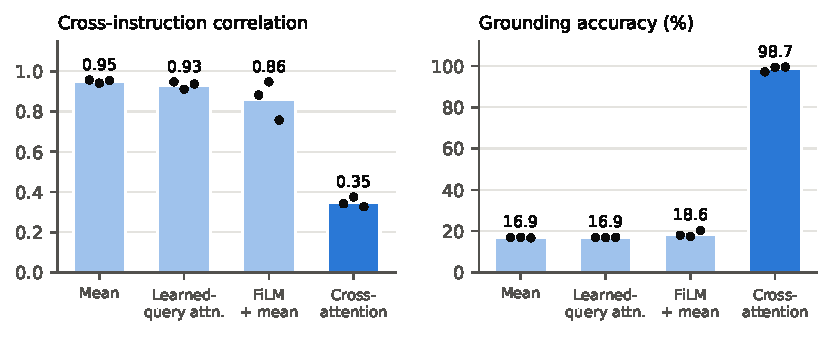
\includegraphics[width=0.82\linewidth]{figures/pooling.pdf}
\caption{Held-out test scenes (300 scenes, 1\,785 instructions). Bars show means
over three training seeds; dots show individual seeds. Chance grounding
accuracy is 16.8\%.}
\label{fig:pool}
\end{figure}

\begin{table}[t]
\centering\small
\begin{tabular}{lccc}
\toprule
Pooling & Cross-instr.\ correlation $\downarrow$ & Grounding acc.\ $\uparrow$ & Median error (mm) $\downarrow$\\
\midrule
Mean & 0.951 $\pm$ 0.008 & 16.9\% $\pm$ 0.2 & 128.7\\
Attention (learned query) & 0.932 $\pm$ 0.019 & 16.9\% $\pm$ 0.1 & 129.0\\
FiLM + mean & 0.863 $\pm$ 0.096 & 18.6\% $\pm$ 1.5 & 125.4\\
Cross-attention & \textbf{0.348 $\pm$ 0.025} & \textbf{98.7\% $\pm$ 1.3} & \textbf{4.5}\\
\bottomrule
\end{tabular}
\caption{Pooling comparison, mean $\pm$ standard deviation over three seeds,
all trained for 12 epochs.}
\label{tab:pool}
\end{table}

Cross-attention pooling lowers the cross-instruction correlation from 0.951
(mean pooling) to 0.348, a \textbf{63\% reduction}. It is also the only
variant that learns the task within the 12-epoch budget: 98.7\% grounding
accuracy and a 4.5\,mm median error, against chance level (16.8\%) for every
other variant (Figure~\ref{fig:pool}, Table~\ref{tab:pool}). The learned-query
attention baseline rules out ``more parameters'' or ``attention in general''
as the explanation: with a fixed query it behaves like mean pooling. What
matters is that the \emph{instruction} chooses what to attend to.

The FiLM baseline is also instruction-aware, yet it barely moves from chance
within 12 epochs. Mean pooling forces it to represent ``where the named object
is'' as an average over all objects, which is a much harder function to learn.
To check whether this is just slow learning, I trained FiLM and mean pooling
for 40 epochs (one seed each). FiLM does learn, slowly: 50.4\% grounding
accuracy after 20 epochs and 60.7\% after 40, with a 49\,mm median error,
still far below cross-attention after 12 epochs. Mean pooling, by contrast, stays at chance (17.3\%) after 40 epochs, even
though its cross-instruction correlation falls to 0.59 and FiLM's to 0.43.
So cross-attention is not the only pooling that can work, but it is far easier
to learn: the instruction picks out one object directly, instead of the
network having to cancel out every other object inside an average.

\textbf{Two cautions.} First, correlation and accuracy are not the same thing.
After 40 epochs, mean pooling's correlation falls to 0.59 while its accuracy
stays at chance, so a lower correlation alone is not evidence of better
grounding.
Second, attention weights are not a clean explanation of the decision.
Figure~\ref{fig:attn} shows a success and a failure on the same scene. Pooled
over three seeds, the error rate is highest when the target is a cylinder
(2.8\%, against 0.9\% for cubes and 0.3\% for balls), because an upright
cylinder seen from above looks like a ball or a cube.

\begin{figure}[t]
\centering
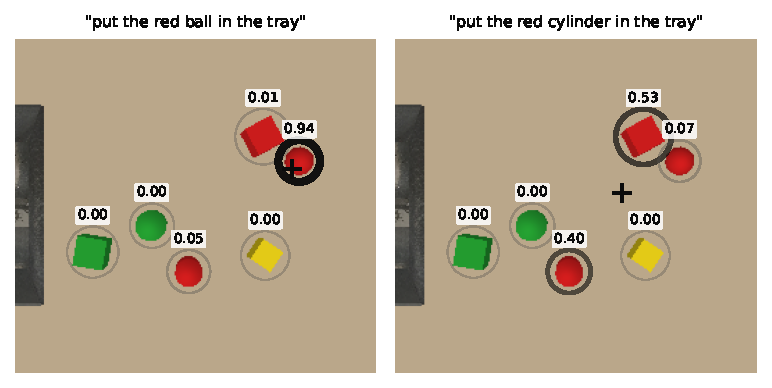
\includegraphics[width=0.74\linewidth]{figures/attention.pdf}
\caption{Cross-attention weights (numbers, ring thickness) and predicted grasp
point ($+$) on one test scene. Left: the weight concentrates on the red ball
and the prediction lands on it. Right: for the red cylinder (lower red object)
the weight is split between the cylinder (0.40) and the red cube (0.53), and the
prediction falls between them, a grounding failure.}
\label{fig:attn}
\end{figure}

\subsection{The learned policy inside the robot loop}
Replacing the hand-written grounder with each trained policy (seed-0
checkpoint) and running the full pick-and-place loop on 100 new cluttered
scenes (seeds 4000--4099) gives the same ranking. Cross-attention succeeds in
\textbf{94\%} of episodes (95\% interval 87.5--97.2) with 5 wrong-object steps.
Mean, learned-query and FiLM pooling succeed in 8\%, 8\% and 6\% of episodes,
with 110 or more wrong-object steps each. The hand-written attribute grounder
still does better (99\%). In this closed world of six colours and three shapes,
a few hand-written rules beat a learned model. The learned policy's advantage
would show only with object descriptions the rules cannot express.


\section{Limitations}
\begin{itemize}\itemsep0pt
\item \textbf{Easy world.} The objects are rigid primitives, grasps are top-down
only, and the camera sees everything from above. High success here says little
about real objects, occlusion or a real robot.
\item \textbf{Closed vocabulary.} The default grounder knows six colours and
three shapes, and its thresholds were tuned by hand on development scenes. The
CLIP grounder is implemented but could not be evaluated, and the LLM planner is
optional and unevaluated. Open-vocabulary grounding and LLM planning are
therefore not tested here.
\item \textbf{Small learned model.} The grounding policy uses the pipeline's own
detections as tokens and is trained for 12 epochs. Baselines were compared at
equal training budget. Given more epochs, FiLM pooling partly catches up (see
Section~5.3).
\item \textbf{Metric.} Cross-instruction correlation is defined in Section~4. As
the FiLM result shows, it should always be reported together with a task metric.
\end{itemize}

\section{Conclusion}
A simple modular pipeline with two targeted fixes, colour splitting of merged
detections and clearance-aware finger placement, picks and places named objects
in 99--100\% of unseen simulated scenes. Its main weakness is its complete trust
in camera calibration: beyond about 10\,mm of error, grasps start to miss. In a controlled comparison, letting the instruction form the attention
query made a small policy learn to ground instructions quickly and accurately. It lowers
the correlation between representations of different instructions by 63\% and
lifts grounding accuracy from chance to 98.7\%. The natural next steps are to
evaluate the open-vocabulary CLIP grounder and LLM planner, add realistic object
meshes and side-on grasps, and test the learned policy on descriptions the
hand-written rules cannot express.

\paragraph{AI use.} The code and this report were developed with AI assistance
(Claude). I directed the work and take responsibility for the results.

\small
\begin{thebibliography}{9}\setlength{\itemsep}{0pt}
\bibitem{pybullet} E.~Coumans, Y.~Bai. PyBullet, a Python module for physics simulation for games, robotics and machine learning. \url{http://pybullet.org}, 2016--2021.
\bibitem{clip} A.~Radford et al. Learning transferable visual models from natural language supervision. \emph{ICML}, 2021.
\bibitem{owlvit} M.~Minderer et al. Simple open-vocabulary object detection with vision transformers. \emph{ECCV}, 2022.
\bibitem{saycan} M.~Ahn et al. Do as I can, not as I say: Grounding language in robotic affordances. \emph{CoRL}, 2022.
\bibitem{cliport} M.~Shridhar, L.~Manuelli, D.~Fox. CLIPort: What and where pathways for robotic manipulation. \emph{CoRL}, 2021.
\bibitem{rt2} A.~Brohan et al. RT-2: Vision-language-action models transfer web knowledge to robotic control. \emph{CoRL}, 2023.
\bibitem{attention} A.~Vaswani et al. Attention is all you need. \emph{NeurIPS}, 2017.
\bibitem{settransformer} J.~Lee et al. Set Transformer: A framework for attention-based permutation-invariant neural networks. \emph{ICML}, 2019.
\bibitem{film} E.~Perez et al. FiLM: Visual reasoning with a general conditioning layer. \emph{AAAI}, 2018.
\end{thebibliography}



\end{document}
